\usepackage{fontspec}
\setmainfont{DejaVu Sans}[Scale=0.86]
\setsansfont{DejaVu Sans}[Scale=0.86]
\usepackage[a4paper,top=2.0cm,bottom=1.8cm,left=1.9cm,right=1.9cm]{geometry}
\usepackage{graphicx}
\usepackage{xcolor}
\usepackage{tikz}
\usetikzlibrary{calc}
\usepackage{enumitem}
\usepackage{fancyhdr}
\usepackage{titlesec}
\usepackage{array}
\usepackage{tabularx}
\usepackage{booktabs}
\usepackage[hidelinks]{hyperref}
\hypersetup{pdfauthor={Dawid Cekała — Ampere Point}, pdfcreator={Ampere Point}}
\usepackage{needspace}

\definecolor{apnavy}{HTML}{1A1A1A}
\definecolor{apnavy2}{HTML}{4A4A4A}
\definecolor{apink}{HTML}{1C2430}
\definecolor{apmuted}{HTML}{5B6675}
\definecolor{apline}{HTML}{E3E3E3}
\definecolor{apbg}{HTML}{F7F7F7}
\definecolor{apgreen}{HTML}{1F8A4C}
\definecolor{apgreenbg}{HTML}{E7F5EC}
\definecolor{apwarn}{HTML}{B9791B}
\definecolor{apwarnbg}{HTML}{FBF1DE}
\definecolor{apaccent}{HTML}{EC6434}

\setlength{\parindent}{0pt}
\setlength{\parskip}{0.35em}
\renewcommand{\arraystretch}{1.25}

\pagestyle{fancy}\fancyhf{}
\renewcommand{\headrulewidth}{0pt}
\renewcommand{\footrulewidth}{0pt}
\providecommand{\DOCAUTH}{oprac. Dawid Cekała}
\fancyfoot[L]{\footnotesize\color{apmuted}\DOCFOOT{} \textperiodcentered{} \DOCAUTH}
\fancyfoot[R]{\footnotesize\color{apmuted}\thepage}

% --- wordmark (placeholder do czasu otrzymania pliku logo) ---
\newcommand{\apwordmark}[1][1]{
\includegraphics[height=\dimexpr #1\dimexpr 0.86cm\relax\relax]{logo_ap.png}}

% --- pasek tytulowy ---
\newcommand{\apheader}[2]{%
\noindent\begin{tikzpicture}
  \node[anchor=north west, inner sep=0pt] at (0,0) {\apwordmark[1.15]};
\end{tikzpicture}\hfill
\raisebox{0.20cm}{\parbox[t]{9.2cm}{\raggedleft\footnotesize\color{apmuted}#2}}\\[0.25cm]
{\color{apaccent}\rule{\textwidth}{1.8pt}}\\[0.30cm]
{\fontspec{DejaVu Sans}\bfseries\color{apnavy}\LARGE #1}\\[0.15cm]}

% --- krok: numer w kolku ---
\newcommand{\kroknum}[1]{%
\tikz[baseline=(k.base)]{\node[circle, fill=apaccent, text=white, inner sep=0pt, minimum size=6.2mm,
  font=\fontspec{DejaVu Sans}\bfseries\small] (k) {#1};}}

% --- ramka informacyjna ---
\newcommand{\apinfo}[2]{%
\par\vspace{0.15cm}
\noindent\begin{tikzpicture}
\node[draw=apline, fill=apbg, line width=0.7pt, rounded corners=5pt, inner sep=8pt,
      text width=\dimexpr\textwidth-2\fboxsep-14pt\relax, align=left]
 {\small\textbf{\color{apnavy}#1}\par\vspace{2pt}\color{apink}#2};
\end{tikzpicture}\par\vspace{0.15cm}}

\newcommand{\apwarnbox}[2]{%
\par\vspace{0.15cm}
\noindent\begin{tikzpicture}
\node[draw=apwarn!45, fill=apwarnbg, line width=0.7pt, rounded corners=5pt, inner sep=8pt,
      text width=\dimexpr\textwidth-2\fboxsep-14pt\relax, align=left]
 {\small\textbf{\color{apwarn}#1}\par\vspace{2pt}\color{apink}#2};
\end{tikzpicture}\par\vspace{0.15cm}}

\newcommand{\apokbox}[2]{%
\par\vspace{0.15cm}
\noindent\begin{tikzpicture}
\node[draw=apgreen!40, fill=apgreenbg, line width=0.7pt, rounded corners=5pt, inner sep=8pt,
      text width=\dimexpr\textwidth-2\fboxsep-14pt\relax, align=left]
 {\small\textbf{\color{apgreen}#1}\par\vspace{2pt}\color{apink}#2};
\end{tikzpicture}\par\vspace{0.15cm}}

% --- komorka kroku: obrazek + opis ---
% #1 numer, #2 tytul, #3 opis, #4 plik
\newcommand{\krok}[4]{%
\begin{minipage}[t]{0.485\textwidth}
  \vspace{0pt}
  \begin{center}\includegraphics[width=\linewidth, height=7.0cm, keepaspectratio]{#4}\end{center}
  \vspace{0.12cm}
  {\kroknum{#1}\ \textbf{\color{apnavy}#2}}\par\vspace{0.05cm}
  {\small\color{apink}#3}
\end{minipage}}

\newcommand{\krokbezobrazka}[3]{%
\begin{minipage}[t]{0.485\textwidth}
  \vspace{0pt}
  \begin{center}
  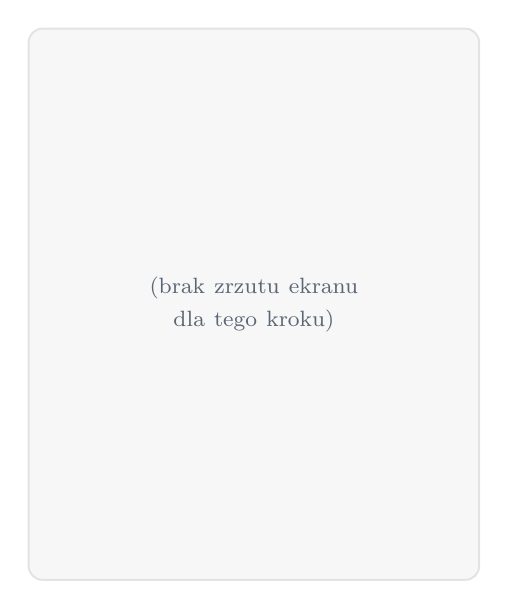
\begin{tikzpicture}
    \node[draw=apline, fill=apbg, line width=0.7pt, rounded corners=5pt, inner sep=6pt,
          minimum height=7.0cm, text width=5.3cm, align=center]
      {\footnotesize\color{apmuted}(brak zrzutu ekranu\\dla tego kroku)};
  \end{tikzpicture}
  \end{center}
  \vspace{0.12cm}
  {\kroknum{#1}\ \textbf{\color{apnavy}#2}}\par\vspace{0.05cm}
  {\small\color{apink}#3}
\end{minipage}}

% --- os czasu doby: #1 etykieta, #2 lista stref blokady "a/b,c/d"
\newcommand{\osczasu}[2]{%
\begin{tikzpicture}[x=0.62cm, y=1cm]
  \fill[apgreenbg, rounded corners=2pt] (0,0) rectangle (24,0.66);
  \foreach \a/\b in {#2}{ \fill[apwarnbg] (\a,0) rectangle (\b,0.66);
      \draw[apwarn, line width=0.8pt] (\a,0) rectangle (\b,0.66);}
  \draw[apline, line width=0.8pt, rounded corners=2pt] (0,0) rectangle (24,0.66);
  \foreach \h in {0,2,...,24}{ \draw[apline, line width=0.5pt] (\h,0) -- (\h,-0.08);
     \node[below, font=\tiny\color{apmuted}] at (\h,-0.06) {\h};}
  \node[left, font=\small\bfseries\color{apnavy}] at (-0.35,0.33) {#1};
\end{tikzpicture}}
